\documentclass{beamer}
\usetheme[hideothersubsections]{AUTheme}
\usefonttheme[]{serif}
\usepackage{pgf,pgfpages,epic,eepic}
\usepackage{graphicx}
\usepackage{amsmath, latexsym, color, amssymb, here}
\usepackage{epsf, epsfig, pifont,tikz,subfigure}
\usepackage{graphics, calrsfs}
\usepackage{times}
\usepackage{fancybox,calc}
\usepackage{palatino,mathpazo}
\usepackage{pgfplots}
%------------------------------------------------------------
	\title{PGFplots}
	\author{Chandru Periasamy}
	\institute{Department of Mechanical Engineerig\\
						Auburn University}
	\date{\today}
\begin{document}
\maketitle
%----------------------------------------------------------frame1
\section{Introduction}
\begin{frame}	
	\frametitle{Introduction to PGFplots}
	PGFplots...\\
	\begin{itemize}
	\item provides tools to generate plots
	\item is built completely on Ti\textit{k}Z/PGF
	\item helps maintain consistency of document and font type/size
	\item claims to be user-friendly !\ (\textit{Really ?!})\\ \pause
	\textit{YES, after you master the 238 page manual !} \pause
	\item I would rather do it on MATLAB\\[20pt]
	\end{itemize}
	\centering{\emph{\color {blue} Nevertheless, PGFplots produces good quality plots}}
\end{frame}
%------------------------------------------------------------frame2
\section{The basics}
\begin{frame}
	\frametitle{The basics}
	These are mandatory
	\begin{itemize}
	\item \color{blue}{ \textbackslash usepackage\{pgfplots\}} \color{black}in the preamble \pause
	\item \color{blue} \textbackslash begin\{tikzpicture\}\\
				\color{blue} \textbackslash begin\{axis\}\\
				...\\
				\color{blue} \textbackslash end\{axis\}\\
				\color{blue} \textbackslash end\{tikzpicture\} \color{black}within the document\\
	\end{itemize}
\end{frame}
%--------------------------------------------------------------frame3
\section{A simple plot}
\begin{frame}[fragile]
\frametitle{A simple (scatter) plot}
\begin{columns}
\column{0.5\textwidth}
\begin{block}{Plot}
\centering{
		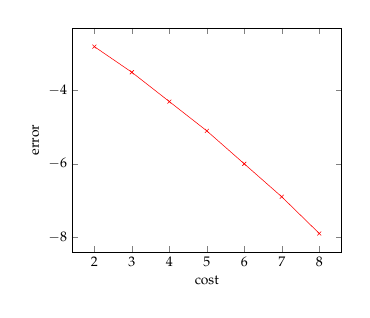
\begin{tikzpicture}[scale=0.5]
		\begin{axis}[
		xlabel=cost, 
		ylabel=error
		]
		\addplot[color=red, mark=x] coordinates{
			(2, -2.8)
			(3, -3.5)
			(4, -4.3)
			(5, -5.1)
			(6, -6)
			(7, -6.9)
			(8, -7.9)
			};
			\end{axis}
		\end{tikzpicture}
		}
\end{block}
\column{0.4\textwidth}
\begin{block}{Code}
\tiny{
\begin{verbatim}
\begin{tikzpicture}
		\begin{axis}[
			xlabel=cost, 
			ylabel=error
			]
		\addplot[color=red, mark=x]
		coordinates{
			(2, -2.8)
			(3, -3.5)
			(4, -4.3)
			(5, -5.1)
			(6, -6)
			(7, -6.9)
			(8, -7.9)
\end{verbatim}
			{\color{blue}\};}
\begin{verbatim}
			\end{axis}
		\end{tikzpicture}
\end{verbatim}
}
\end{block}
\end{columns}
\end{frame}
%-----------------------------------------------
\section{Ploting expressions}
\begin{frame}[fragile]
\frametitle{Ploting expressions}
\begin{columns}
\column{0.5\textwidth}
\begin{block}{Plot}
\centering{
	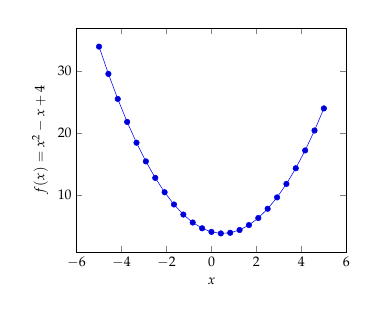
\begin{tikzpicture}[scale=0.5]
		\begin{axis}[
			xlabel=$x$, 
			ylabel={$f(x)=x^2-x+4$}
			]
		\addplot{x^2-x+4};
		\end{axis}
		\end{tikzpicture}	
		}
\end{block}
\column{0.4\textwidth}
\begin{block}{Code}
\centering{
\tiny{
\begin{verbatim}
\begin{tikzpicture}
		\begin{axis}[
		xlabel=$x$, 
		ylabel={$f(x)=x^2-x+4$}
		]
\end{verbatim}
{\color{blue}\textbackslash addplot\{x\^{}2-x+4\};}
\begin{verbatim}
			\end{axis}
		\end{tikzpicture}
		\end{verbatim}
		}
}
\end{block}
\end{columns}
\end{frame}
%------------------------------------------------------------------
\section{Multiple plots \& Legend}
\begin{frame}[fragile]
\frametitle{Multiple plots \& Legend}
\begin{columns}
\column{0.5\textwidth}
\begin{block}{Plot}
\centering{
	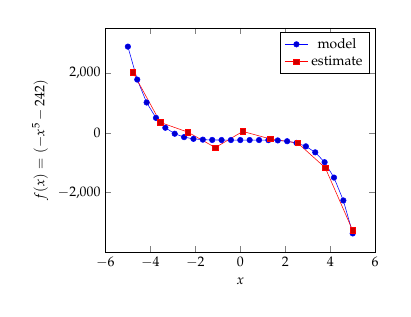
\begin{tikzpicture}[scale=0.5]
		\begin{axis}[
		xlabel=$x$, 
		ylabel={$f(x)=(-x^5-242)$}
		]
		\addplot{-x^5-242};
		\addlegendentry{model}
		\addplot coordinates{
		(-4.77778,2027.60977)
		(-3.55556,347.84069)
		(-2.33333,22.58953)
		(-1.11111,-493.50066)
		(0.11111,46.66082)
		(1.33333,-205.56286)
		(2.55556,-341.40638)
		(3.77778,-1169.24780)
		(5.00000,-3269.56775)
		};
		\addlegendentry{estimate}
		
		\end{axis}
		\end{tikzpicture}	
		}
	\end{block}
\column{0.4\textwidth}
\begin{block}{Code}
\tiny{
\begin{verbatim}
	\begin{tikzpicture}
		\begin{axis}[
		xlabel=$x$, 
		ylabel={$f(x)=(-x^5-242)$}
		]
		\addplot{-x^5-242};
\end{verbatim}
		{\color{blue}\textbackslash addlegendentry\{model\}}
\begin{verbatim}
		\addplot coordinates{
		(-4.77778,2027.60977)
		(-3.55556,347.84069)
		(-2.33333,22.58953)
		(-1.11111,-493.50066)
		(0.11111,46.66082)
		(1.33333,-205.56286)
		(2.55556,-341.40638)
		(3.77778,-1169.24780)
		(5.00000,-3269.56775)
		};
\end{verbatim}
		{\color{blue}\textbackslash addlegendentry\{estimate\}}
\begin{verbatim}
		\end{axis}
		\end{tikzpicture}
\end{verbatim}
		}
	\end{block}
\end{columns}
\end{frame}
%---------------------------------------------------------
\begin{frame}[fragile]
\frametitle{Easy legend entry}
\begin{columns}
\column{0.5\textwidth}
\begin{block}{Plot}
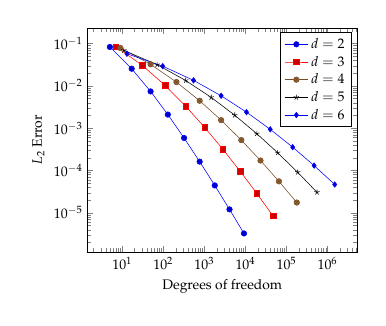
\begin{tikzpicture}[scale=0.5]
	\begin{loglogaxis}[
	xlabel={Degrees of freedom},
	ylabel={$L_2$ Error}
	]
		\addplot coordinates {
		(5,8.312e-02) (17,2.547e-02) (49,7.407e-03)
		(129,2.102e-03) (321,5.874e-04) (769,1.623e-04)
		(1793,4.442e-05) (4097,1.207e-05) (9217,3.261e-06)
		};
		\addplot coordinates{
		(7,8.472e-02) (31,3.044e-02) (111,1.022e-02)
		(351,3.303e-03) (1023,1.039e-03) (2815,3.196e-04)
		(7423,9.658e-05) (18943,2.873e-05) (47103,8.437e-06)
		};
		\addplot coordinates{
		(9,7.881e-02) (49,3.243e-02) (209,1.232e-02)
		(769,4.454e-03) (2561,1.551e-03) (7937,5.236e-04)
		(23297,1.723e-04) (65537,5.545e-05) (178177,1.751e-05)
		};
		\addplot coordinates{
		(11,6.887e-02) (71,3.177e-02) (351,1.341e-02)
		(1471,5.334e-03) (5503,2.027e-03) (18943,7.415e-04)
		(61183,2.628e-04) (187903,9.063e-05) (553983,3.053e-05)
		};
		\addplot coordinates{
		(13,5.755e-02) (97,2.925e-02) (545,1.351e-02)
		(2561,5.842e-03) (10625,2.397e-03) (40193,9.414e-04)
		(141569,3.564e-04) (471041,1.308e-04) (1496065,4.670e-05)
		};
		\legend{$d=2$,$d=3$,$d=4$,$d=5$,$d=6$}
	\end{loglogaxis}
\end{tikzpicture}
\end{block}
\column{0.4\textwidth}
\begin{block}{Code}
\tiny{
\begin{verbatim}
\begin{tikzpicture}
	\begin{loglogaxis}[
	xlabel={Degrees of freedom},
	ylabel={$L_2$ Error}
	]
		\addplot coordinates {
		(5,8.312e-02). . .  
		(129,2.102e-03). . . 
		(1793,4.442e-05). . .
		};
		\addplot coordinates{
		. . .
		};
		\addplot coordinates{
		. . .
		};
		\addplot coordinates{
		. . .
		};
		\addplot coordinates{
		. . .
		};
\end{verbatim}
{\color{blue}\textbackslash legend\{\$d=2\$,\$d=3\$,\$d=4\$,\$d=5\$,\$d=6\$\}}
\begin{verbatim}
	\end{loglogaxis}
\end{tikzpicture}
\end{verbatim}
}
\end{block}
\end{columns}
\end{frame}
%----------------------------------------------------------------
\section{Log axis}
\begin{frame}[fragile]
\frametitle{Log axis}
\begin{columns}
\column{0.5\textwidth}
\begin{block}{Plot}
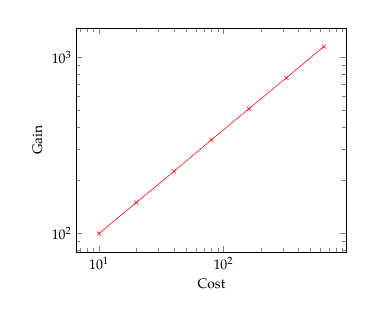
\begin{tikzpicture}[scale=0.5]
	\begin{loglogaxis}[xlabel=Cost,ylabel=Gain]
	\addplot[color=red,mark=x] coordinates {
		(10,100)
		(20,150)
		(40,225)
		(80,340)
		(160,510)
		(320,765)
		(640,1150)
		};
	\end{loglogaxis}
\end{tikzpicture}
\end{block}
\column{0.4\textwidth}
\begin{block}{Code}
\tiny{
\begin{verbatim}
\begin{tikzpicture}
\end{verbatim}
	{\color{blue}\textbackslash begin\{loglogaxis\}}
\begin{verbatim}
	[xlabel=Cost,ylabel=Gain]
	\addplot[color=red,mark=x]
		coordinates {
		(10,100)
		(20,150)
		(40,225)
		(80,340)
		(160,510)
		(320,765)
		(640,1150)
		};
	\end{loglogaxis}
\end{tikzpicture}
\end{verbatim}
}
\end{block}
\end{columns}
\end{frame}
%-------------------------------------------------------------
\begin{frame}[fragile]
\frametitle{Semilog axis}
\begin{columns}
\column{0.5\textwidth}
\begin{block}{Plot}
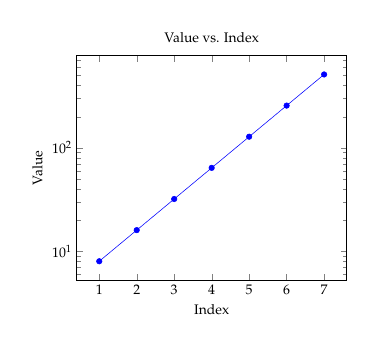
\begin{tikzpicture}[scale=0.5,]
	\begin{semilogyaxis}[
		xlabel=Index,ylabel=Value,title=Value vs. Index]
		\addplot[color=blue,mark=*] coordinates {
		(1,8)
		(2,16)
		(3,32)
		(4,64)
		(5,128)
		(6,256)
		(7,512)
		};
	\end{semilogyaxis}
	\end{tikzpicture}
\end{block}
\column{0.4\textwidth}
\begin{block}{Code}
\tiny{
\begin{verbatim}
\begin{tikzpicture}
\end{verbatim}
	{\color{blue}\textbackslash begin\{semilogyaxis\}}
[xlabel=Index,ylabel=Value,\\
{\color{blue}title=Value vs. Index]}
\begin{verbatim}
		\addplot[color=blue,mark=*]
		coordinates {
		(1,8)
		(2,16)
		(3,32)
		(4,64)
		(5,128)
		(6,256)
		(7,512)
		};
	\end{semilogyaxis}
	\end{tikzpicture}
\end{verbatim}
}
\end{block}
\end{columns}
\end{frame}
%----------------------------------------------------------------
\section{Bar plots}
\begin{frame}[fragile]
\frametitle{Bar plots}
\begin{columns}
\column{0.5\textwidth}
\begin{block}{Plot}
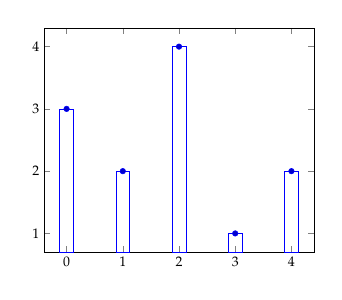
\begin{tikzpicture}[scale=0.5]
	\begin{axis}
		\addplot+[ybar] plot coordinates
		{(0,3) (1,2) (2,4) (3,1) (4,2)};
	\end{axis}
	\end{tikzpicture}
\end{block}
\column{0.4\textwidth}
\begin{block}{Code}
\tiny{
\begin{verbatim}
\begin{tikzpicture}
	\begin{axis}
\end{verbatim}
		{\color{blue}\textbackslash addplot+[ybar]} plot coordinates
\begin{verbatim}
		{(0,3) (1,2) (2,4) (3,1) (4,2)};
	\end{axis}
	\end{tikzpicture}
\end{verbatim}
}
\end{block}
\end{columns}
\end{frame}
%-------------------------------------------------------------
\section{Axis limits}
\begin{frame}[fragile]
\frametitle{Axis limits (domain)}
\begin{columns}
\column{0.5\textwidth}
\begin{block}{Plot}
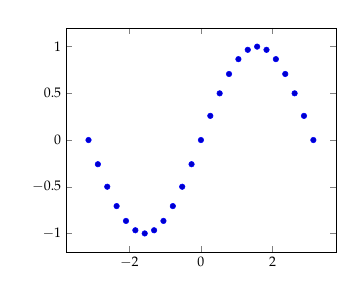
\begin{tikzpicture}[scale=0.5]
	\begin{axis}
		\addplot+[only marks,domain=-pi:pi]
		{sin(deg(x))};
	\end{axis}
	\end{tikzpicture}
\end{block}
\column{0.4\textwidth}
\begin{block}{Code}
\tiny{
\begin{verbatim}
\begin{tikzpicture}
	\begin{axis}
\end{verbatim}
		\textbackslash addplot+[{\color{blue}only marks,domain=-pi:pi}]
\begin{verbatim}
		{sin(deg(x))};
	\end{axis}
	\end{tikzpicture}
\end{verbatim}
}
\end{block}
\end{columns}
\end{frame}
%-------------------------------------------------------------
\section{Error bars}
\begin{frame}[fragile]
\frametitle{Error bars}
\begin{columns}
\column{0.5\textwidth}
\begin{block}{Plot}
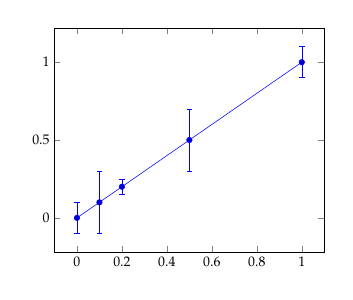
\begin{tikzpicture}[scale=0.5]
	\begin{axis}
		\addplot plot[error bars/.cd,
		y dir=both, y explicit]
		coordinates{
		(0,0) +- (0.5,0.1)
		(0.1,0.1) +- (0.05,0.2)
		(0.2,0.2) +- (0,0.05)
		(0.5,0.5) +- (0.1,0.2)
		(1,1) +- (0.3,0.1)
		};
	\end{axis}
	\end{tikzpicture}
\end{block}
\column{0.4\textwidth}
\begin{block}{Code}
\tiny{
\begin{verbatim}
\begin{tikzpicture}
	\begin{axis}
\end{verbatim}
		\textbackslash addplot {\color{blue}plot[error bars/.cd,\\
		y dir=both{\color{red}(plus/minus)}, y explicit]}
\begin{verbatim}
		coordinates{
		(0,0) +- (0.5,0.1)
		(0.1,0.1) +- (0.05,0.2)
		(0.2,0.2) +- (0,0.05)
		(0.5,0.5) +- (0.1,0.2)
		(1,1) +- (0.3,0.1)
		};
	\end{axis}
	\end{tikzpicture}
\end{verbatim}
}
\end{block}
\end{columns}
\end{frame}
%-------------------------------------------------------------
\section{3D plots}
\begin{frame}[fragile]
\frametitle{3D plots}
\begin{columns}
\column{0.5\textwidth}
\begin{block}{Plot}
\begin{figure}[h!]
	\centering
	\includegraphics[width=4cm]{surf.png}
\end{figure}
\end{block}
\column{0.4\textwidth}
\begin{block}{Code}
\tiny{
\begin{verbatim}
\begin{tikzpicture}
	\begin{axis}
\end{verbatim}
		\textbackslash {\color{blue}addplot3[surf,domain=0:360,samples=40]}
\begin{verbatim}
		{sin(x)*sin(y)};
	\end{axis}
	\end{tikzpicture}
\end{verbatim}
}
\end{block}
\end{columns}
\end{frame}
%--------------------------------------------------------------------
\begin{frame}[fragile]
\vfill
\centering{Thank You}
\vfill
\end{frame}
\end{document}

